%%%%%%%%%%%%%%%%%%%%%%%%%%%%%%%%%%%%%%%%%
% University/School Laboratory Report
% LaTeX Template
% Version 3.1 (25/3/14)
%
% This template has been downloaded from:
% http://www.LaTeXTemplates.com
%
% Original author:
% Linux and Unix Users Group at Virginia Tech Wiki 
% (https://vtluug.org/wiki/Example_LaTeX_chem_lab_report)
%
% License:
% CC BY-NC-SA 3.0 (http://creativecommons.org/licenses/by-nc-sa/3.0/)
%
%%%%%%%%%%%%%%%%%%%%%%%%%%%%%%%%%%%%%%%%%

%----------------------------------------------------------------------------------------
%	PACKAGES AND DOCUMENT CONFIGURATIONS
%----------------------------------------------------------------------------------------

\documentclass{article}

\usepackage[version=3]{mhchem} % Package for chemical equation typesetting
\usepackage{siunitx} % Provides the \SI{}{} and \si{} command for typesetting SI units
\usepackage{graphicx} % Required for the inclusion of images
\usepackage{natbib} % Required to change bibliography style to APA
\usepackage{amsmath} % Required for some math elements 
\usepackage{enumitem}
\usepackage{hyperref}
\setlength\parindent{0pt} % Removes all indentation from paragraphs

\renewcommand{\labelenumi}{\alph{enumi}.} % Make numbering in the enumerate environment by letter rather than number (e.g. section 6)

%\usepackage{times} % Uncomment to use the Times New Roman font

%----------------------------------------------------------------------------------------
%	DOCUMENT INFORMATION
%----------------------------------------------------------------------------------------

\title{Report \\ Analysis of University Rankings} % Title

\author{Julian \textsc{Backé} \\ Tobias \textsc{Salzer} \\ Ajayvir \textsc{Singh}} % Author name

\date{January 21, 2020} % Date for the report

\begin{document}

\maketitle % Insert the title, author and date

% If you wish to include an abstract, uncomment the lines below
% \begin{abstract}
% Abstract text
% \end{abstract}

%----------------------------------------------------------------------------------------
%	SECTION 1
%----------------------------------------------------------------------------------------

\section{Objective}

The objective of this project is to analyse, visualise and interpret data concerning university rankings. Certain characteristics of universities, such as their publication history, research output, number of students, budget, ... are considered for this task. Furthermore, the characteristics of countries and regions these universities are located in, are analysed to determine how those characteristics influence the rankings of said universities.
\pagebreak
%----------------------------------------------------------------------------------------
%	SECTION 2
%----------------------------------------------------------------------------------------
\section{Workflow}

\begin{enumerate}[label=\textbf {\arabic*.}]
\item \textbf{Problem definition:} \\ 
How do university rankings change over time? Which characteristics of universities contribute most to good rankings, or to large changes in the ranking position? Are there predictors for increases or decreases in the rankings?

\item \textbf{Data acquisition:} \\
\begin{enumerate}[label=\textbf {\alph*)}]
\item The main source of data for the rankings itself based on certain characteristics of the university:
\hypertarget{World University Rankings}{} \href{https://www.kaggle.com/mylesoneill/world-university-rankings\#cwurData.csv}{\textbf{World University Rankings}}

\item Although missing a substantial amount of data, the \href{https://www.kaggle.com/mylesoneill/world-university-rankings\#shanghaiData.csv}{\textbf{Shanghai dataset}} for world rankings was useful, because it contained data starting from 2005.

\item Similarly, the \href{https://www.kaggle.com/mylesoneill/world-university-rankings\#timesData.csv}{\textbf{Times dataset}} contained data not in the previous two datasets, allowing us to retrieve information about the number of students, ratio to staff etc.

\item To gain information about expenditure, we found it necessary to use the \href{https://www.kaggle.com/mylesoneill/world-university-rankings\#education_expenditure_supplementary_data.csv}{\textbf{Expenditure dataset}}.

\item Since previous datasets only contained data about characteristics of the universities itself, the following data set contains data about a characteristic of the country itself: \href{https://www.kaggle.com/tjysdsg/human-development-index\#Human\%20Development\%20Index.csv}{\textbf{Human Development Index}}

\item To analyse rankings over regions, a way to order countries by region was necessary. The following dataset of countries ordered by region was used: \href{https://www.kaggle.com/fernandol/countries-of-the-world\#countries of the world.csv}{\textbf{Countries of the world}}

\item Another feature that was planned to be considered was a measure of corruption by country:
\href{https://www.kaggle.com/transparencyint/corruption-index\#history.csv}{\textbf{Corruption Perceptions Index}}

%TODO: add remaining dataset links and description
\end{enumerate}
\item \textbf{Data loading:} \\
The next step was to preload data into separate dataframes:
%TODO: Insert code piece here?

\item \textbf{Preprocessing data:} \\
One of the challenges of this analysis was to bring all the different datasets into a unified format. This included renaming certain columns and values, imputing missing values, removing unnecessary columns and stripping white-spaces.

\begin{enumerate}[label=\textbf {\alph*)}]
	
\item \textbf{Renaming:}\\One issue was different naming schemes for certain data. Analysing and renaming such values was imperative before merging data.
%TODO: insert preprocessing code here?

\item \textbf{Missing data:}
\\Similarly, we discovered that some datasets had missing data.
\\Shanghai dataset contained a column, which had over 75\% missing values. Due this specific characteristic (score) being contained in another dataset already, it was decided to completely remove this column.
%TODO: code of data removal here?
\\Our main dataset, the \hyperlink{name}{\textbf{World University Rankings}}, seemed relative complete, with the exception of some missing values for  \emph{broad\_impact} characteristic. By analysing how many rows were missing and the correlation to ranking of universities, we came to the conclusion, that multivariate imputation would be an optimal solution here, due to good correlation with other characteristics and only a small amount of rows being required to be imputed, leading to introduction of almost no bias.
For instance, we see that \emph{broad\_impact} characteristic has a very good correlation with the rankings:

\begin{figure}[h]
	\centering
	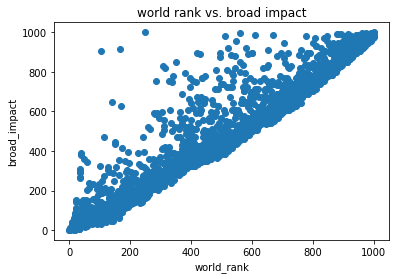
\includegraphics[width=10cm,height=10cm,keepaspectratio]{graphs/impact_rank_scatterplot}
	\caption{world rank vs broad impact.}
	\label{fig:impact_rank_scatterplot}
\end{figure}

%TODO: code of data imputation here?
\item \textbf{...}


\end{enumerate}

\item \textbf{Data Exploration}

\item \textbf{Data Modelling}
\end{enumerate}
\pagebreak

%----------------------------------------------------------------------------------------
%	SECTION 3
%----------------------------------------------------------------------------------------
\section{Data Exploration}

\subsection{Correlation Matrix for World University Rankings}

We found it effective to construct a heatmap to get a general overview of how characteristics of universities correlate with their rankings and which correlate the most:

\begin{figure}[h]
\centering
		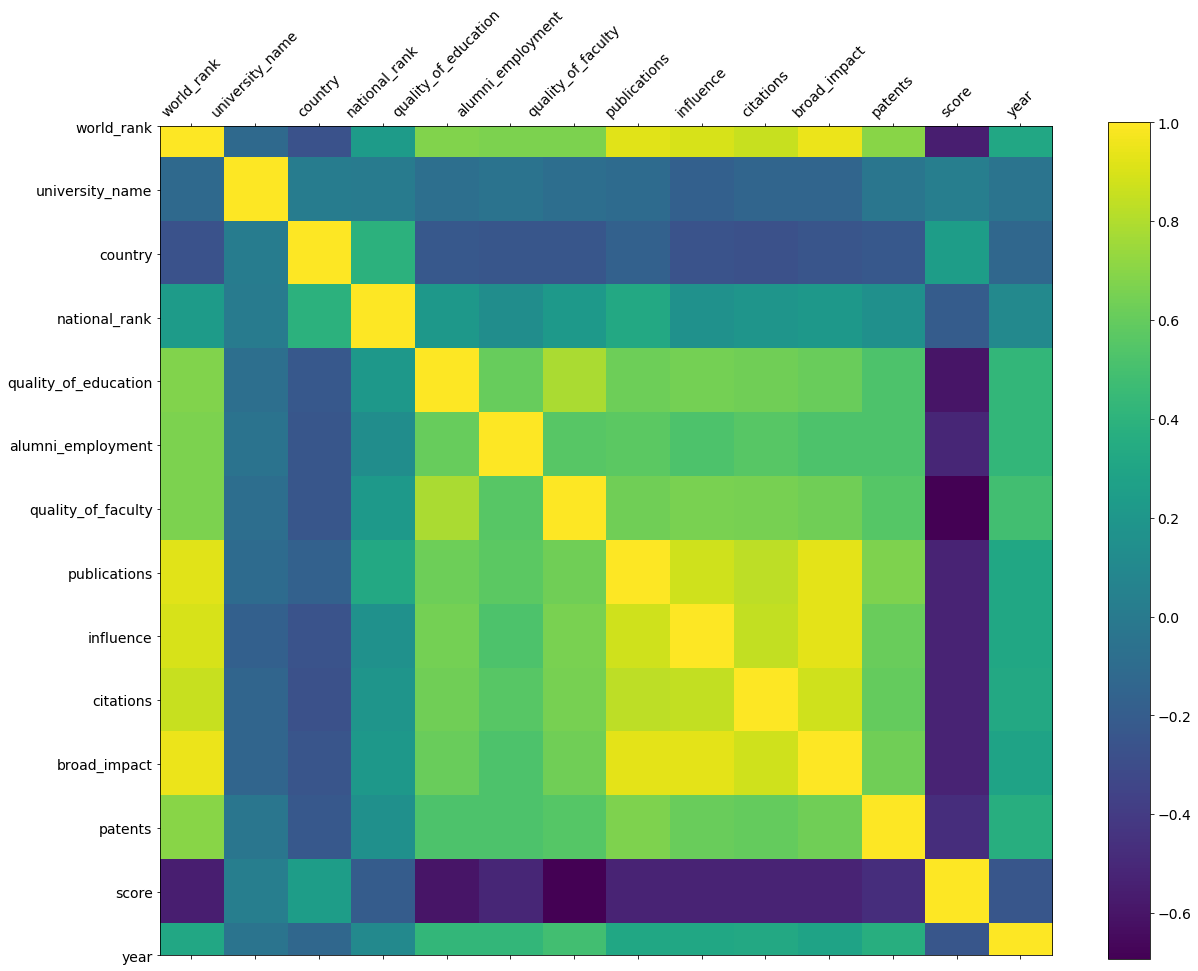
\includegraphics[width=10cm,height=10cm,keepaspectratio]{graphs/world_uni_hm}
		\caption{World University Rankings Heatmap.}
\end{figure}

As evident, while certain characteristics contribute less to a good rank, others, like \emph{broad\_impact}, have a surprisingly good correlation with the rank. It is evident, that imputing  \emph{broad\_impact} could have introduced some bias to the data, but as shown in Figure ~\ref{fig:impact_rank_scatterplot}, the correlation between these two characteristics was already good before.
\section{...}


%----------------------------------------------------------------------------------------
%	SECTION 4
%----------------------------------------------------------------------------------------

\section{...}

\section{Results and Conclusions}

%----------------------------------------------------------------------------------------
%	BIBLIOGRAPHY
%----------------------------------------------------------------------------------------

\bibliographystyle{apalike}

\bibliography{sample}

%----------------------------------------------------------------------------------------


\end{document}